\documentclass[12pt,a4paper]{article}

\usepackage[utf8]{inputenc}
\usepackage[spanish]{babel}
\usepackage{graphicx}
\usepackage{geometry}
\geometry{a4paper, margin=2.5cm}
\usepackage{xcolor}
\usepackage{listings}
\usepackage{booktabs}
\usepackage{amsmath}
\usepackage{subcaption}
\usepackage{float}
\usepackage[colorlinks=true, linkcolor=blue, urlcolor=blue]{hyperref}

\definecolor{codegreen}{rgb}{0,0.6,0}
\definecolor{codegray}{rgb}{0.5,0.5,0.5}
\definecolor{codepurple}{rgb}{0.58,0,0.82}
\definecolor{backcolour}{rgb}{0.95,0.95,0.92}

\lstdefinestyle{mystyle}{
    backgroundcolor=\color{backcolour},   
    commentstyle=\color{codegreen},
    keywordstyle=\color{magenta},
    numberstyle=\tiny\color{codegray},
    stringstyle=\color{codepurple},
    basicstyle=\ttfamily\footnotesize,
    breakatwhitespace=false,         
    breaklines=true,                 
    captionpos=b,                    
    keepspaces=true,                 
    numbers=left,                    
    numbersep=5pt,                  
    showspaces=false,                
    showstringspaces=false,
    showtabs=false,                  
    tabsize=2,
    literate={á}{{\'a}}1 {é}{{\'e}}1 {í}{{\'i}}1 {ó}{{\'o}}1 {ú}{{\'u}}1
             {Á}{{\'A}}1 {É}{{\'E}}1 {Í}{{\'I}}1 {Ó}{{\'O}}1 {Ú}{{\'U}}1
             {ñ}{{\~n}}1 {Ñ}{{\~N}}1
}
\lstset{style=mystyle}

\title{\Huge\textbf{PROYECTO ESP32} \\ \Large Control de Brillo de LED con Potenciómetro \\ \vspace{0.5cm} \normalsize \textit{Lectura analógica ADC, conversión a voltaje y modulación PWM del brillo de un LED}}
\author{Msc. Néstor Fabio Montoya Palacios}
\date{2026 \\ \vspace{0.2cm} \small Plataforma: ESP32 Dev Module}

\begin{document}

\maketitle
\tableofcontents
\newpage

% ══════════════════════════════════════════════════════════════
\section{Introducción}
% ══════════════════════════════════════════════════════════════

Este documento describe de manera detallada el proyecto ``Control de Brillo de LED con Potenciómetro'', una práctica introductoria de electrónica analógica y digital con el microcontrolador ESP32. El sistema lee la posición angular de un \textbf{potenciómetro} mediante el conversor analógico-digital (ADC) del ESP32, convierte el valor leído en voltaje y en un ciclo de trabajo PWM, y utiliza este último para controlar el \textbf{brillo de un LED} de forma continua y proporcional.

El proyecto introduce conceptos fundamentales de \textbf{lectura analógica con ADC de 12 bits}, \textbf{conversión de valores digitales a magnitudes físicas (voltaje)}, \textbf{modulación por ancho de pulso (PWM)} para el control de actuadores, y \textbf{comunicación serial} para la depuración y monitoreo de datos en tiempo real.

Se trata de una práctica ideal como primer acercamiento a la interacción entre sensores analógicos y actuadores controlados digitalmente, sentando las bases para proyectos más complejos de automatización y control.

% ══════════════════════════════════════════════════════════════
\section{Objetivo del Proyecto}
% ══════════════════════════════════════════════════════════════

Implementar un sistema de control analógico-digital utilizando el microcontrolador ESP32 que lea la posición de un potenciómetro y controle proporcionalmente el brillo de un LED, demostrando el uso de:
\begin{itemize}
    \item Lectura de señales analógicas mediante el ADC de 12 bits del ESP32 (rango 0--4095).
    \item Conversión de valores digitales crudos a magnitudes físicas (voltaje en el rango 0--3,3\,V).
    \item Modulación por ancho de pulso (PWM) con la API \texttt{ledcAttach()} / \texttt{ledcWrite()} del ESP32.
    \item Mapeo lineal entre rangos numéricos distintos con la función \texttt{map()}.
    \item Protección de valores con la función \texttt{constrain()}.
    \item Comunicación serial para monitoreo en tiempo real de las variables del sistema.
\end{itemize}

% ══════════════════════════════════════════════════════════════
\section{Materiales Necesarios}
% ══════════════════════════════════════════════════════════════

\begin{table}[h!]
\centering
\begin{tabular}{cll}
\toprule
\textbf{Cant.} & \textbf{Componente} & \textbf{Especificación} \\
\midrule
1 & ESP32 Dev Module & Microcontrolador dual-core con Wi-Fi/Bluetooth \\
1 & Potenciómetro & 10\,k$\Omega$ lineal, 3 terminales \\
1 & LED rojo & Diodo emisor de luz, 5\,mm, $V_f \approx 2$\,V \\
1 & Resistencia & 220\,$\Omega$ (limitadora de corriente para el LED) \\
1 & Protoboard & Placa de pruebas de 830 puntos \\
  & Cables jumper & Macho-macho para conexiones \\
1 & Cable USB & Para programación y alimentación del ESP32 \\
\bottomrule
\end{tabular}
\caption{Lista de materiales del proyecto Potenciómetro}
\end{table}

% ══════════════════════════════════════════════════════════════
\section{Esquema de Conexión}
% ══════════════════════════════════════════════════════════════

El siguiente esquema, realizado en Fritzing, muestra las conexiones físicas del circuito. El potenciómetro se conecta entre 3,3\,V y GND, con su terminal central (cursor) conectado a GPIO34 del ESP32. El LED se conecta a GPIO4 a través de una resistencia limitadora de 220\,$\Omega$.

\begin{figure}[H]
\centering
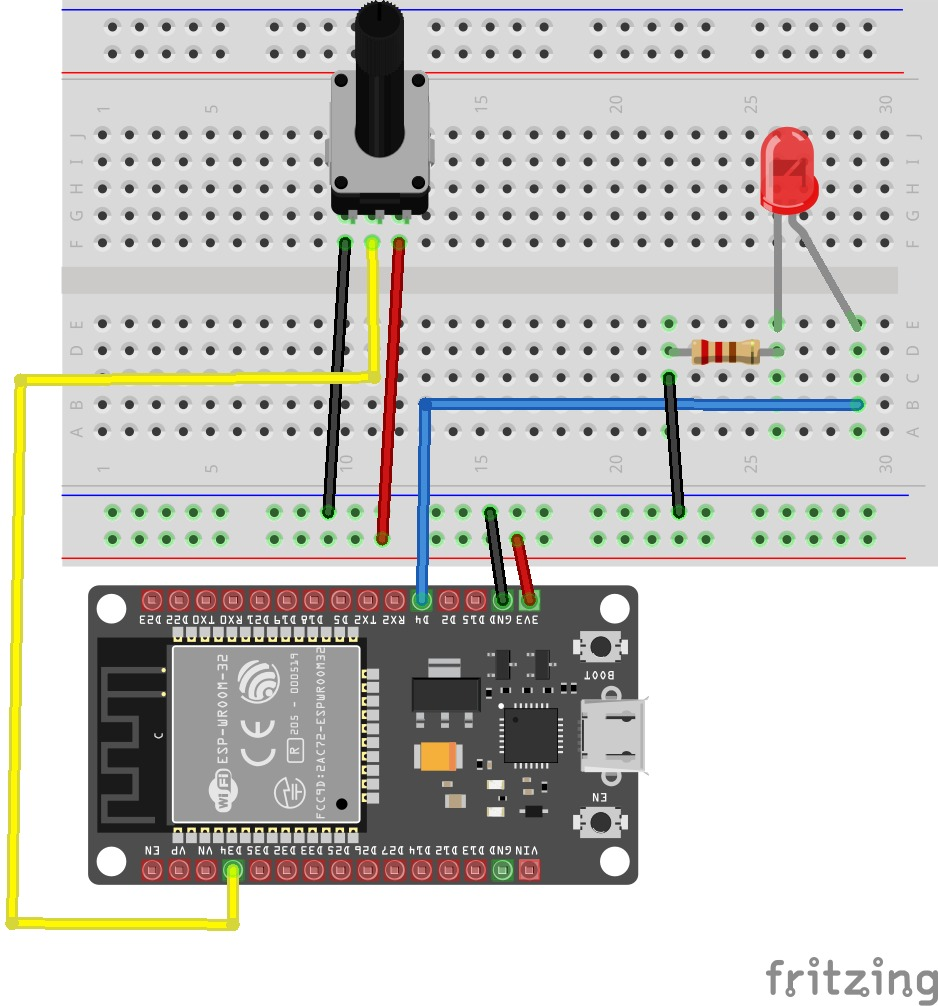
\includegraphics[width=0.85\textwidth]{../Esquemas/Potenciometro_esq.jpeg}
\caption{Esquema de conexión del circuito -- Control de LED con Potenciómetro (Fritzing)}
\label{fig:esquema}
\end{figure}

\subsection{Diagrama de Conexiones}

\begin{center}
\begin{tabular}{lll}
\toprule
\textbf{Componente} & \textbf{Pin} & \textbf{ESP32 GPIO} \\
\midrule
Potenciómetro & Terminal 1 & 3.3V \\
Potenciómetro & Terminal 2 (cursor) & GPIO34 (ADC1\_CH6) \\
Potenciómetro & Terminal 3 & GND \\
Resistencia 220\,$\Omega$ & Terminal 1 & GPIO4 \\
LED rojo & Ánodo (+) & Resistencia 220\,$\Omega$ (Terminal 2) \\
LED rojo & Cátodo (--) & GND \\
\bottomrule
\end{tabular}
\end{center}

\textbf{Nota:} El GPIO34 del ESP32 es un pin de \textit{solo entrada} (input-only), lo que lo hace ideal para lectura analógica ya que no requiere funcionalidad de salida. Este pin pertenece al canal ADC1\_CH6.

% ══════════════════════════════════════════════════════════════
\section{Código Fuente}
% ══════════════════════════════════════════════════════════════

A continuación se presenta el código completo del proyecto. Se ha organizado en secciones funcionales claramente delimitadas por comentarios.

\subsection{Código Completo}
\lstinputlisting[language=C++, title=Potenciometro.ino]{../Arduino/Potenciometro/Potenciometro.ino}

% ══════════════════════════════════════════════════════════════
\subsection{Análisis del Código}
% ══════════════════════════════════════════════════════════════

\subsubsection*{Declaración de Pines}
El programa define dos constantes para los pines de hardware:
\begin{itemize}
    \item \textbf{\texttt{pinPotenciometro = 34}:} GPIO34 del ESP32, configurado como entrada analógica. Este pin pertenece al canal ADC1\_CH6 del conversor analógico-digital. Es un pin de solo entrada (\textit{input-only}), lo que significa que no puede usarse como salida digital ni PWM.
    \item \textbf{\texttt{pinLED = 4}:} GPIO4 del ESP32, utilizado como salida PWM para controlar el brillo del LED.
\end{itemize}

\subsubsection*{Configuración PWM}
La modulación por ancho de pulso se configura con dos parámetros:
\begin{itemize}
    \item \textbf{\texttt{frecuenciaPWM = 5000}:} Frecuencia de la señal PWM fijada en 5\,kHz. Esta frecuencia es suficientemente alta para que el ojo humano no perciba parpadeo en el LED (la frecuencia mínima para evitar \textit{flicker} visible es aproximadamente 100\,Hz).
    \item \textbf{\texttt{resolucionPWM = 8}:} Resolución de 8 bits, lo que proporciona $2^8 = 256$ niveles de brillo (valores de 0 a 255).
\end{itemize}

\subsubsection*{Función \texttt{setup()}}
\begin{enumerate}
    \item Inicia la comunicación serial a 115200 baudios para el monitoreo de datos.
    \item Configura el pin del potenciómetro como entrada con \texttt{pinMode(pinPotenciometro, INPUT)}.
    \item Configura el canal PWM asociado al pin del LED mediante \texttt{ledcAttach(pinLED, frecuenciaPWM, resolucionPWM)}. Esta función de la API moderna del ESP32 (Arduino core $\geq$ 3.x) asocia directamente un pin a un canal PWM con la frecuencia y resolución especificadas.
    \item Imprime un mensaje de bienvenida en el monitor serial.
\end{enumerate}

\subsubsection*{Función \texttt{loop()}}
El bucle principal ejecuta cinco pasos secuenciales en cada iteración:

\begin{enumerate}
    \item \textbf{PASO 1 -- Lectura analógica:} Se lee el valor del potenciómetro con \texttt{analogRead(pinPotenciometro)}. El ADC de 12 bits del ESP32 entrega un entero entre 0 (potenciómetro al mínimo) y 4095 (potenciómetro al máximo).
    
    \item \textbf{PASO 2 -- Conversión a voltaje:} El valor digital crudo se convierte a voltaje mediante la relación lineal:
    \begin{equation}
    V = \frac{\text{valor} \times 3{,}3}{4095}
    \label{eq:voltaje}
    \end{equation}
    donde 3,3\,V es el voltaje de referencia del ADC del ESP32 y 4095 es el valor máximo del ADC de 12 bits ($2^{12} - 1$).
    
    \item \textbf{PASO 3 -- Mapeo a brillo PWM:} La función \texttt{map(valor, 0, 4095, 0, 255)} realiza una interpolación lineal que convierte el rango del ADC (0--4095) al rango del PWM (0--255):
    \begin{equation}
    \text{brillo} = \left\lfloor \frac{\text{valor} \times 255}{4095} \right\rfloor
    \label{eq:brillo}
    \end{equation}
    Adicionalmente, \texttt{constrain(brillo, 0, 255)} asegura que el valor resultante no exceda los límites del PWM.
    
    \item \textbf{PASO 4 -- Aplicación del PWM:} Se escribe el valor de brillo en el canal PWM del LED con \texttt{ledcWrite(pinLED, brillo)}. Un valor de 0 apaga completamente el LED, mientras que 255 lo enciende al máximo brillo.
    
    \item \textbf{PASO 5 -- Monitoreo serial:} Se imprimen en una sola línea el valor crudo del ADC, el voltaje calculado (con 2 decimales) y el valor de brillo PWM.
\end{enumerate}

El ciclo se repite cada 300\,ms (\texttt{delay(300)}) para evitar saturar el monitor serial sin sacrificar la responsividad del control.

% ══════════════════════════════════════════════════════════════
\section{Principio de Funcionamiento}
% ══════════════════════════════════════════════════════════════

\subsection{El Potenciómetro como Divisor de Voltaje}

Un potenciómetro es una resistencia variable de tres terminales que actúa como un \textbf{divisor de voltaje} ajustable. Al conectar sus terminales extremos entre $V_{CC}$ (3,3\,V) y GND, el terminal central (cursor o wiper) entrega un voltaje proporcional a la posición angular del eje:

\begin{equation}
V_{\text{cursor}} = V_{CC} \times \frac{R_2}{R_1 + R_2} = V_{CC} \times \frac{\theta}{\theta_{\max}}
\label{eq:divisor}
\end{equation}

donde $R_1$ y $R_2$ son las resistencias a cada lado del cursor, y $\theta$ es el ángulo de rotación. Así, al girar el potenciómetro de un extremo a otro, el voltaje en el cursor varía linealmente de 0\,V a 3,3\,V.

\subsection{Conversión Analógica-Digital (ADC)}

El ESP32 integra dos módulos ADC (ADC1 y ADC2) con resolución configurable de hasta 12 bits. En este proyecto se utiliza el ADC1 en el canal 6 (GPIO34):

\begin{itemize}
    \item \textbf{Resolución:} 12 bits $\Rightarrow$ $2^{12} = 4096$ niveles (0 a 4095).
    \item \textbf{Voltaje de referencia:} 0 a 3,3\,V.
    \item \textbf{Resolución de voltaje:} $\Delta V = \frac{3{,}3}{4095} \approx 0{,}806$\,mV por nivel.
\end{itemize}

La función \texttt{analogRead()} realiza una conversión SAR (\textit{Successive Approximation Register}) que tarda aproximadamente 2\,$\mu$s, devolviendo un entero proporcional al voltaje de entrada.

\subsection{Modulación por Ancho de Pulso (PWM)}

El PWM es una técnica de control que varía el \textbf{ciclo de trabajo} (\textit{duty cycle}) de una señal cuadrada para controlar la potencia entregada a una carga. El ESP32 dispone de 16 canales PWM independientes implementados por hardware.

El ciclo de trabajo se define como:
\begin{equation}
D = \frac{t_{\text{ON}}}{T} \times 100\,\%
\label{eq:duty}
\end{equation}

donde $t_{\text{ON}}$ es el tiempo en estado alto y $T$ es el período de la señal. Con 8 bits de resolución:

\begin{itemize}
    \item \texttt{brillo = 0} $\Rightarrow$ $D = 0\,\%$ (LED apagado).
    \item \texttt{brillo = 127} $\Rightarrow$ $D \approx 50\,\%$ (LED a media intensidad).
    \item \texttt{brillo = 255} $\Rightarrow$ $D = 100\,\%$ (LED al máximo).
\end{itemize}

A 5\,kHz, el período de la señal PWM es $T = 1/5000 = 200\,\mu$s. El LED se enciende y apaga tan rápidamente que el ojo humano percibe un brillo promedio proporcional al ciclo de trabajo, gracias a la \textit{persistencia retiniana}.

\subsection{Cadena Completa de Procesamiento}

El flujo de datos completo del sistema puede resumirse así:

\begin{verbatim}
    Potenciómetro          ADC 12-bit         Mapeo           PWM 8-bit
    (ángulo)    ──────>   (0 - 4095)   ──────>  map()  ──────>  (0 - 255)
    0° - 270°              voltaje              brillo          duty cycle
                          0 - 3.3 V                            0% - 100%
                                                                  │
                                                                  v
                                                            Brillo del LED
\end{verbatim}

% ══════════════════════════════════════════════════════════════
\section{Fotografías del Montaje}
% ══════════════════════════════════════════════════════════════

Las siguientes imágenes muestran el proyecto montado y en funcionamiento. Se puede observar el ESP32 montado sobre su placa de expansión con borneras de tornillo, el potenciómetro y el LED con su resistencia limitadora conectados en la protoboard.

\begin{figure}[H]
\centering
\begin{subfigure}[b]{0.48\textwidth}
    \centering
    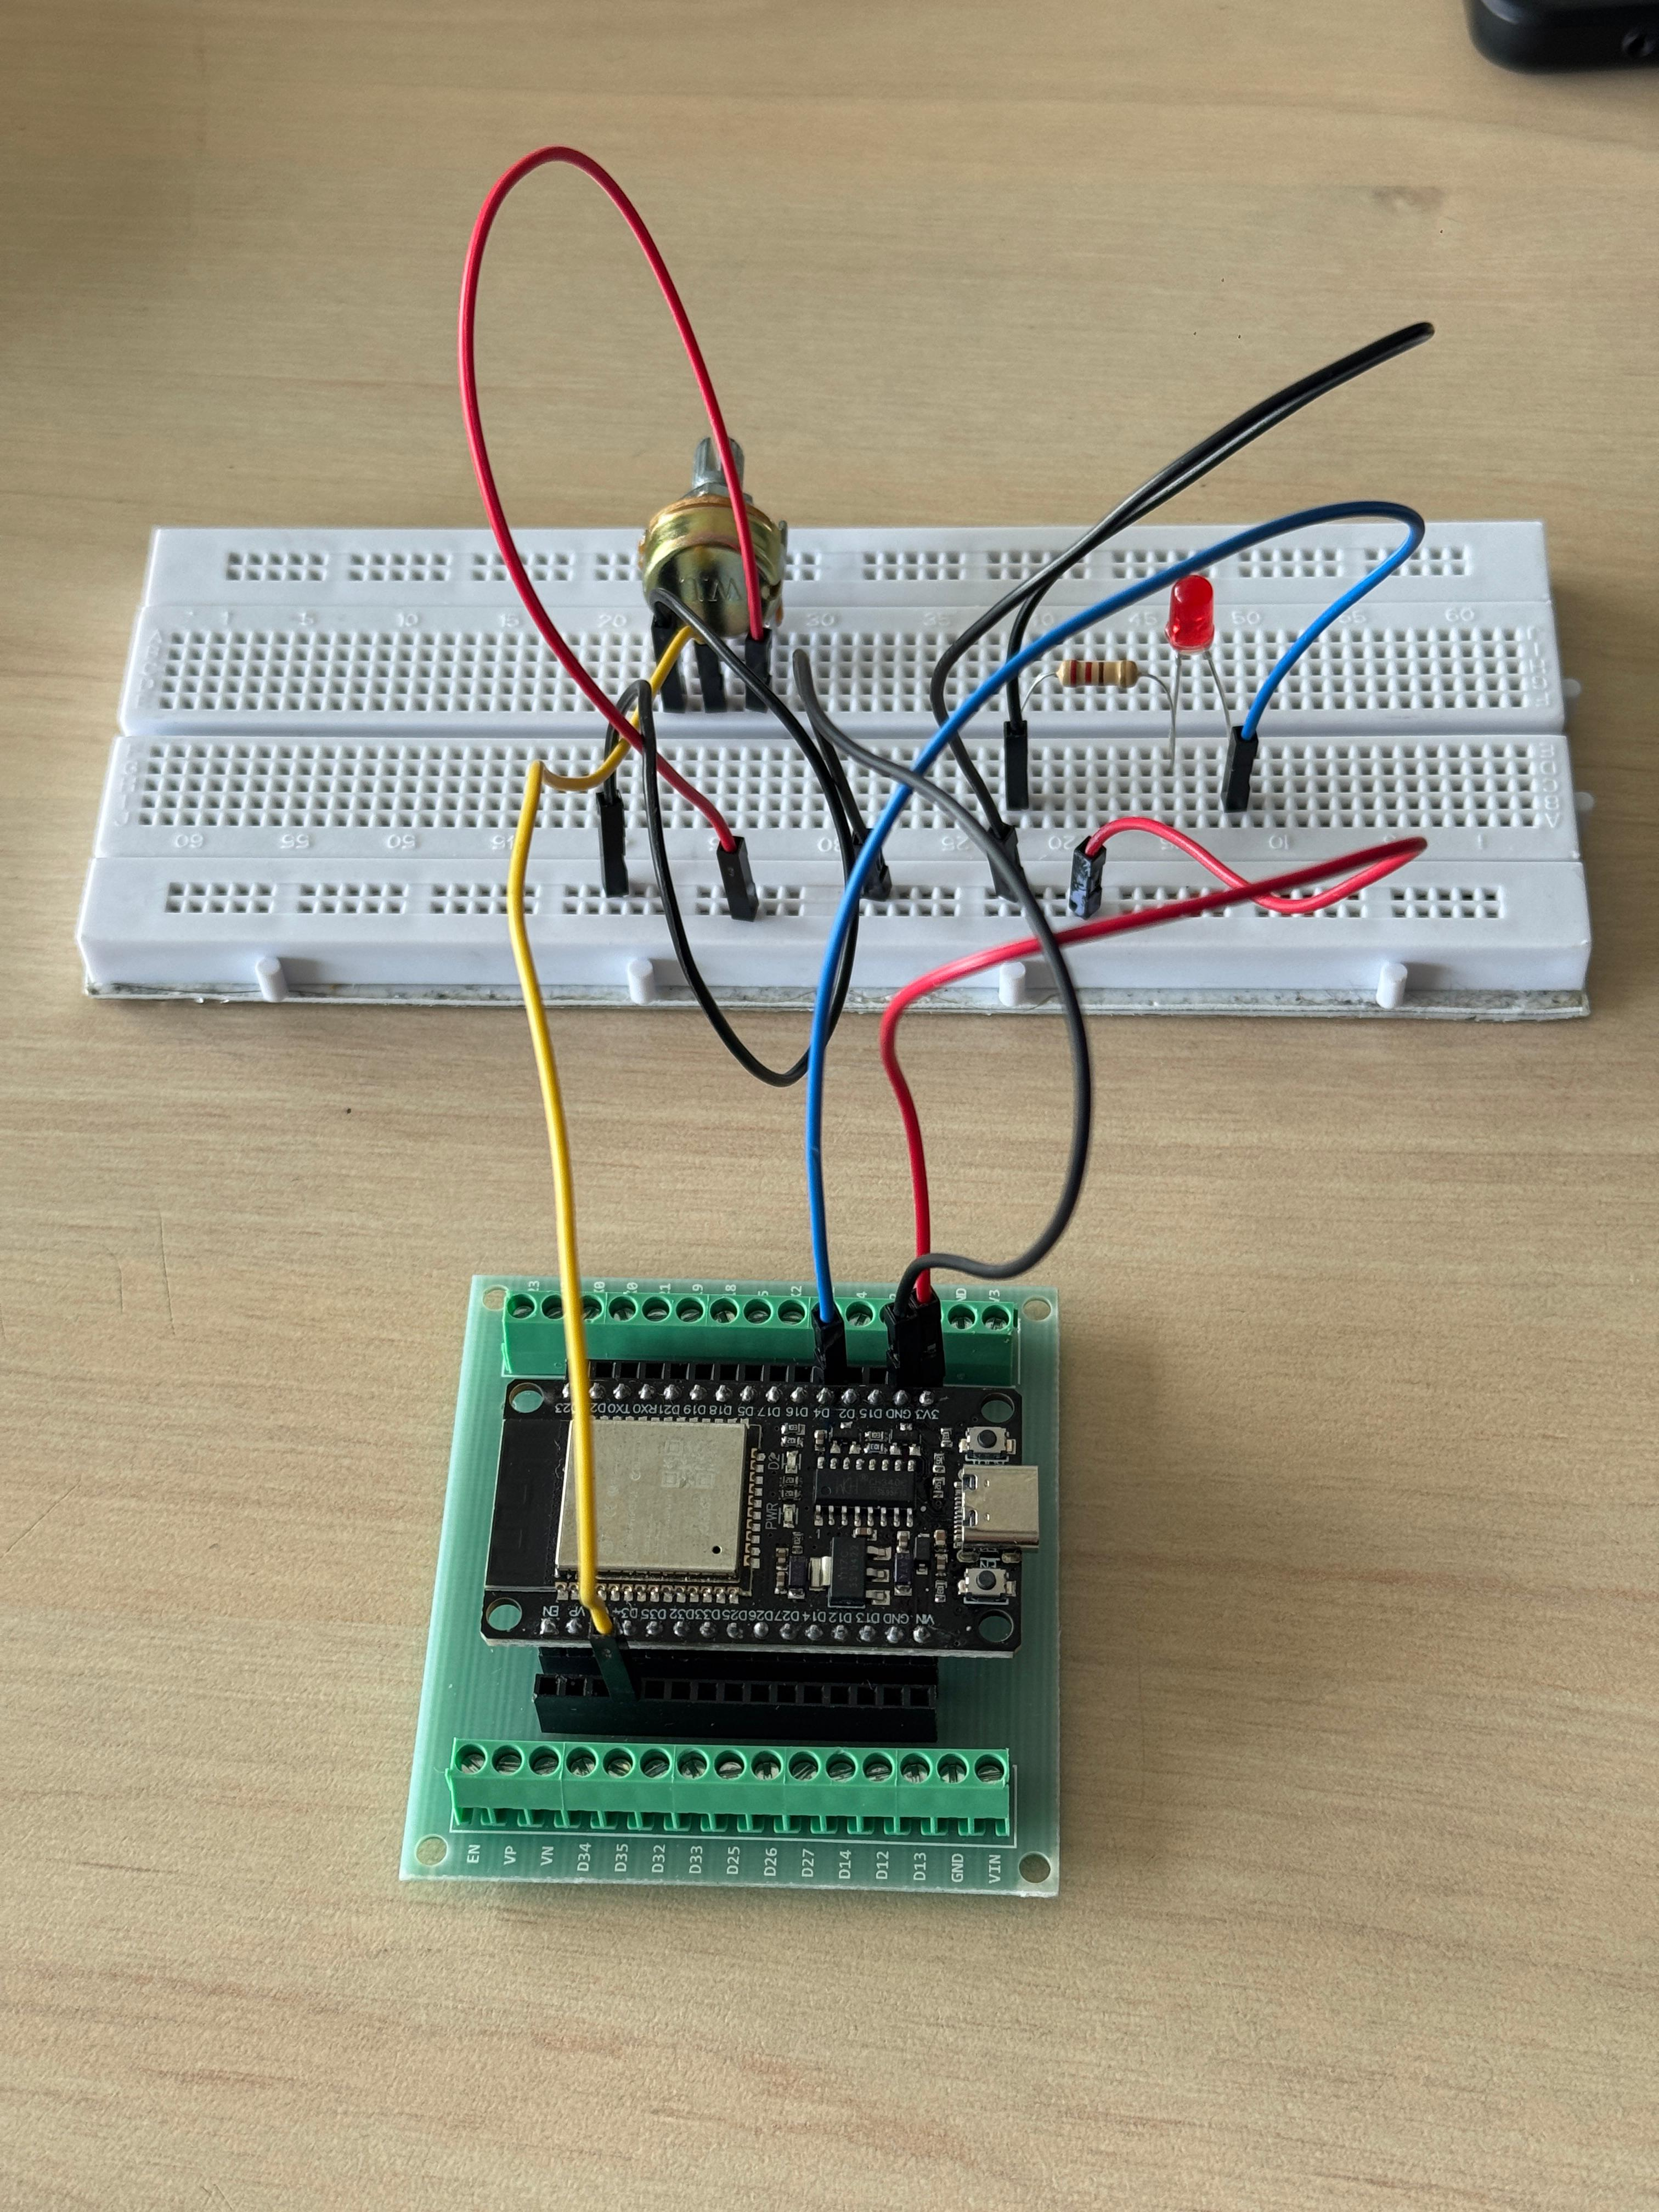
\includegraphics[width=\textwidth]{../Imagenes/Potenciometro_imgs/Potenciometro_img1.jpeg}
    \caption{Vista superior del montaje: ESP32 con placa de expansión, potenciómetro y LED en protoboard}
    \label{fig:montaje1}
\end{subfigure}
\hfill
\begin{subfigure}[b]{0.48\textwidth}
    \centering
    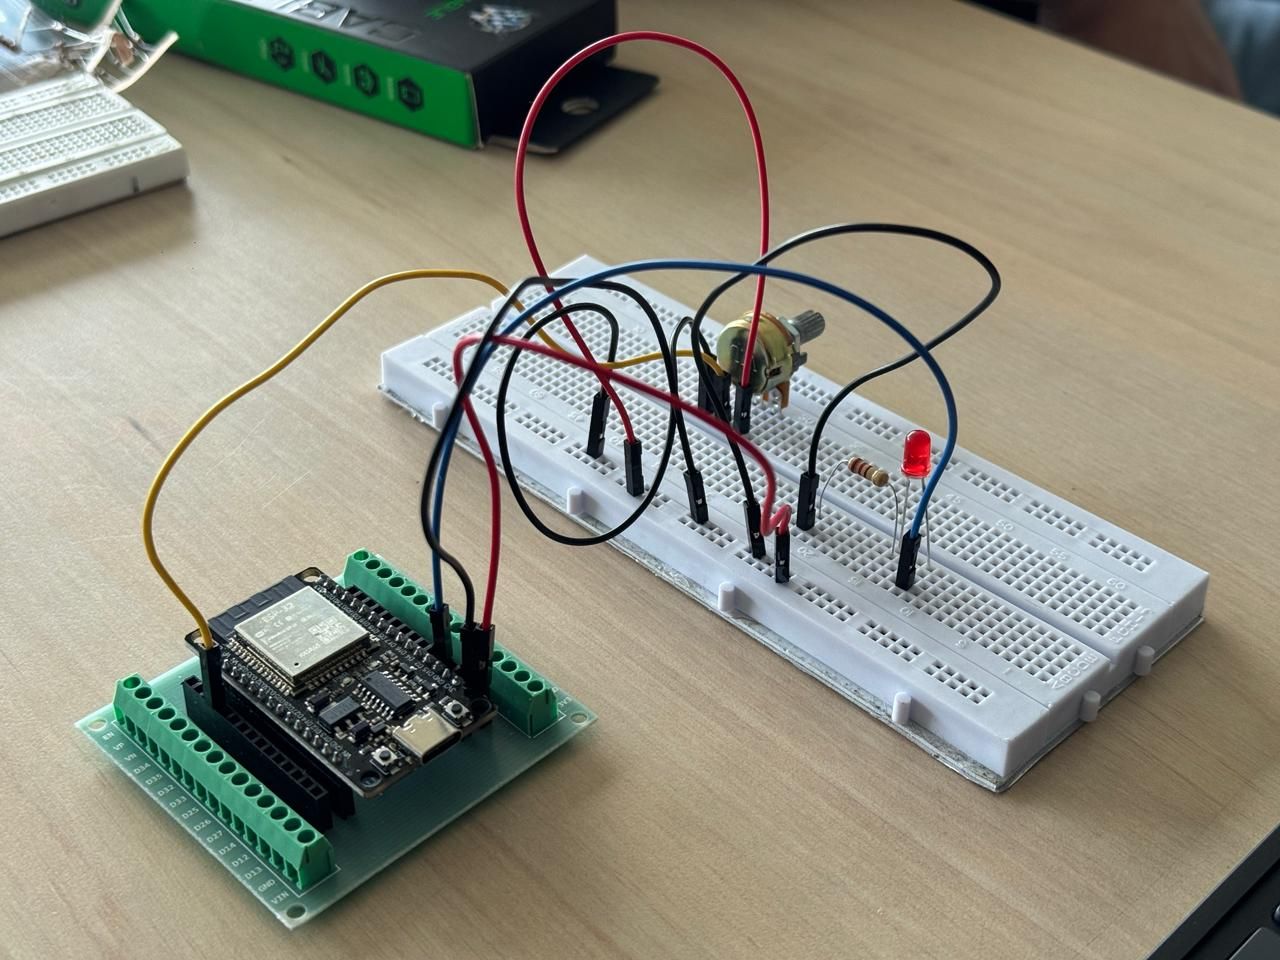
\includegraphics[width=\textwidth]{../Imagenes/Potenciometro_imgs/Potenciometro_img2.jpeg}
    \caption{Vista en perspectiva del circuito mostrando las conexiones de cableado}
    \label{fig:montaje2}
\end{subfigure}
\caption{Montaje físico del proyecto Control de LED con Potenciómetro}
\label{fig:montaje}
\end{figure}

\begin{figure}[H]
\centering
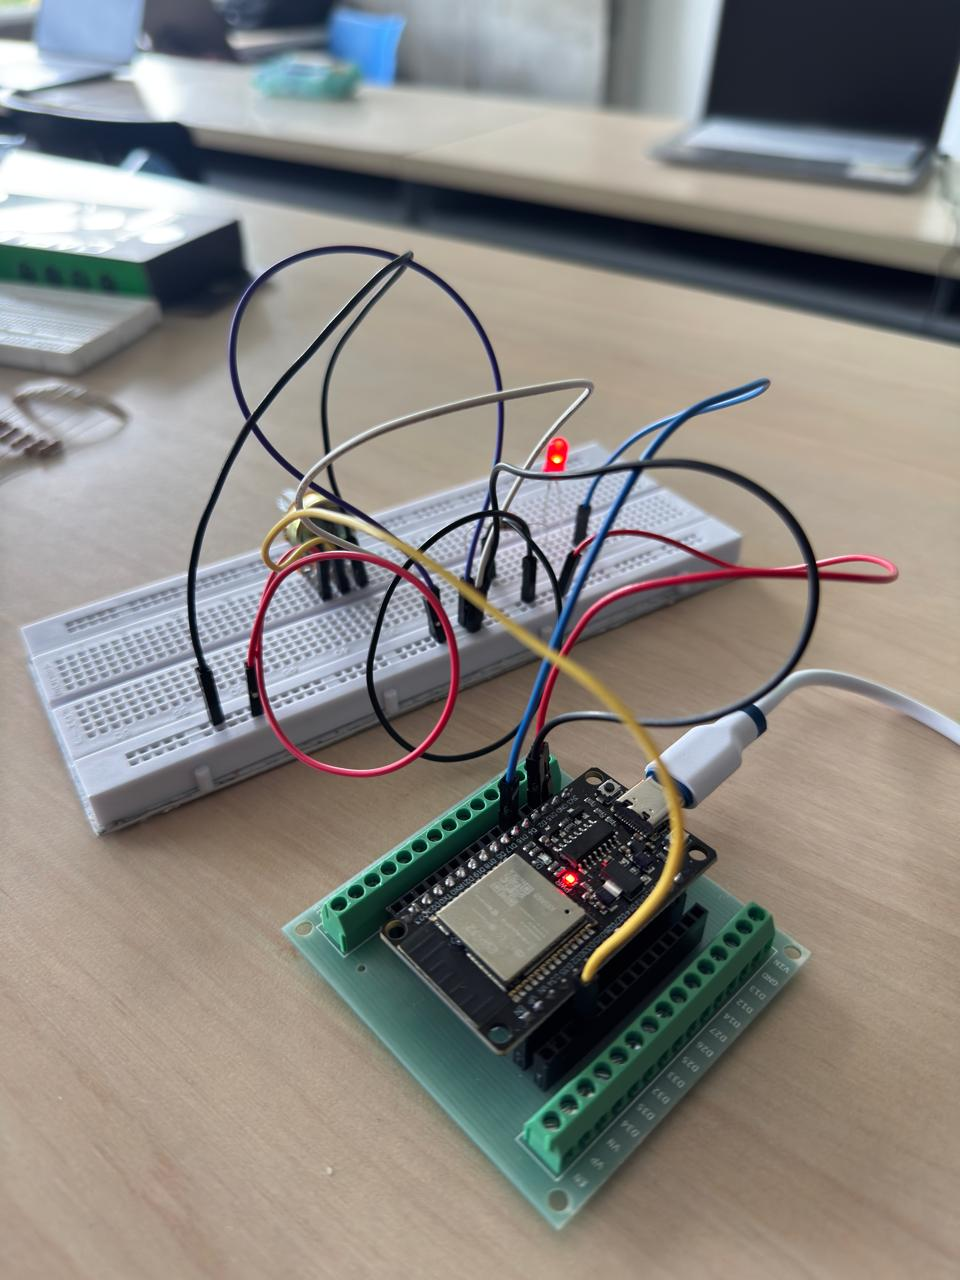
\includegraphics[width=0.6\textwidth]{../Imagenes/Potenciometro_imgs/Potenciometro_img3.jpeg}
\caption{Proyecto en funcionamiento: se observa el LED encendido (indicando que el potenciómetro no está en posición mínima) y el ESP32 conectado vía USB para alimentación y monitoreo serial}
\label{fig:montaje3}
\end{figure}

En la Figura~\ref{fig:montaje3} se aprecia el LED rojo encendido, lo que indica que el potenciómetro se encuentra en una posición intermedia o máxima, entregando un ciclo de trabajo PWM mayor a cero. El cable USB conectado al ESP32 permite tanto la alimentación del circuito como la comunicación serial para monitorear los valores en tiempo real.

% ══════════════════════════════════════════════════════════════
\section{Video de Funcionamiento}
% ══════════════════════════════════════════════════════════════

Se dispone de dos videos que demuestran el funcionamiento del proyecto:

\begin{itemize}
    \item \textbf{Potenciometro\_funcionamiento.mp4}: Demostración básica del control de brillo del LED al girar el potenciómetro.
    \item \textbf{Potenciometro\_funcionamiento2.mp4}: Demostración extendida mostrando el rango completo de variación del brillo, desde apagado total hasta máxima intensidad.
\end{itemize}

Estos videos se encuentran en la carpeta \texttt{Videos/Potenciometro\_vid/} del repositorio del proyecto.

% ══════════════════════════════════════════════════════════════
\section{Proceso de Creación}
% ══════════════════════════════════════════════════════════════

El desarrollo de este proyecto siguió los siguientes pasos:

\begin{enumerate}
    \item \textbf{Selección de componentes:} Se eligió un potenciómetro lineal de 10\,k$\Omega$ por su respuesta proporcional y su compatibilidad con el rango de voltaje del ADC del ESP32 (0--3,3\,V). El LED rojo con resistencia de 220\,$\Omega$ limita la corriente a aproximadamente:
    \begin{equation*}
        I_{LED} = \frac{V_{GPIO} - V_f}{R} = \frac{3{,}3 - 2{,}0}{220} \approx 5{,}9\,\text{mA}
    \end{equation*}
    valor seguro tanto para el LED como para el GPIO del ESP32 (máximo 40\,mA por pin).
    
    \item \textbf{Diseño del circuito:} Se diseñó el esquema en Fritzing (Figura~\ref{fig:esquema}), seleccionando GPIO34 para la entrada analógica (pin de solo entrada, ADC1\_CH6) y GPIO4 para la salida PWM del LED.
    
    \item \textbf{Montaje en protoboard:} Se realizó el cableado físico siguiendo el esquema, conectando el potenciómetro como divisor de voltaje y el LED en serie con la resistencia limitadora.
    
    \item \textbf{Programación:} Se desarrolló el firmware en Arduino IDE con la siguiente estructura lógica:
    \begin{itemize}
        \item Declaración de constantes de hardware (pines, frecuencia PWM, resolución).
        \item Configuración inicial: serial, pin de entrada, canal PWM.
        \item Bucle principal: lectura ADC $\rightarrow$ conversión a voltaje $\rightarrow$ mapeo a PWM $\rightarrow$ escritura al LED $\rightarrow$ impresión serial.
    \end{itemize}
    
    \item \textbf{Configuración del Arduino IDE:}
    \begin{itemize}
        \item Placa: \textit{ESP32 Dev Module}.
        \item Velocidad de subida: 115200 baudios.
        \item Puerto: COM correspondiente al ESP32 conectado.
    \end{itemize}
    
    \item \textbf{Pruebas y validación:} Se verificó el correcto funcionamiento girando el potenciómetro en todo su rango y observando la variación proporcional del brillo del LED, así como los valores en el monitor serial.
\end{enumerate}

% ══════════════════════════════════════════════════════════════
\section{Conceptos Técnicos Clave}
% ══════════════════════════════════════════════════════════════

\subsection{API PWM del ESP32 (Arduino Core 3.x)}

A partir del Arduino Core 3.x para ESP32, la API de PWM se simplificó significativamente. Las funciones antiguas \texttt{ledcSetup()} y \texttt{ledcAttachPin()} fueron reemplazadas por:

\begin{itemize}
    \item \texttt{ledcAttach(pin, frecuencia, resolución)}: Configura y asocia un canal PWM a un pin GPIO en una sola llamada.
    \item \texttt{ledcWrite(pin, dutyCycle)}: Escribe el ciclo de trabajo directamente al pin (ya no se referencia por número de canal).
\end{itemize}

\subsection{Función \texttt{map()}}

La función \texttt{map()} realiza una interpolación lineal entre dos rangos:

\begin{equation}
\text{salida} = \frac{(x - \text{in\_min}) \times (\text{out\_max} - \text{out\_min})}{\text{in\_max} - \text{in\_min}} + \text{out\_min}
\label{eq:map}
\end{equation}

En este proyecto: $\texttt{map(valor, 0, 4095, 0, 255)}$ convierte el rango del ADC de 12 bits al rango del PWM de 8 bits.

\subsection{Función \texttt{constrain()}}

La función \texttt{constrain(x, min, max)} limita un valor al rango $[\text{min}, \text{max}]$:

\begin{equation*}
\texttt{constrain}(x, a, b) = \begin{cases} a & \text{si } x < a \\ x & \text{si } a \leq x \leq b \\ b & \text{si } x > b \end{cases}
\end{equation*}

Se usa como medida de seguridad para garantizar que el valor de brillo nunca exceda el rango válido del PWM (0--255), aunque en este caso \texttt{map()} ya debería producir valores dentro del rango.

% ══════════════════════════════════════════════════════════════
\section{Conclusiones}
% ══════════════════════════════════════════════════════════════

\begin{itemize}
    \item El proyecto demuestra la cadena completa de procesamiento analógico-digital: desde la lectura de un sensor analógico (potenciómetro) hasta el control de un actuador (LED) mediante PWM.
    \item El ADC de 12 bits del ESP32 proporciona una resolución de aproximadamente 0,8\,mV por nivel, suficiente para aplicaciones de control analógico de precisión moderada.
    \item La modulación PWM a 5\,kHz con 8 bits de resolución permite 256 niveles de brillo perceptualmente continuos, sin parpadeo visible para el ojo humano.
    \item La función \texttt{map()} simplifica enormemente la conversión entre rangos numéricos diferentes, siendo una herramienta fundamental en la programación de microcontroladores.
    \item El uso de \texttt{constrain()} como medida defensiva ilustra una buena práctica de programación: validar los rangos de las variables antes de enviarlas al hardware.
    \item La comunicación serial permite depurar y verificar el comportamiento del sistema en tiempo real, mostrando simultáneamente el valor crudo del ADC, el voltaje calculado y el valor PWM aplicado.
    \item Este proyecto sienta las bases para aplicaciones más complejas como control de motores, regulación de temperatura, interfaces hombre-máquina y sistemas de automatización.
\end{itemize}

\end{document}
